\section{Processing Pipeline}
\begin{figure*}[!h]
\begin{center}
\subfigure[]{
    \centering
    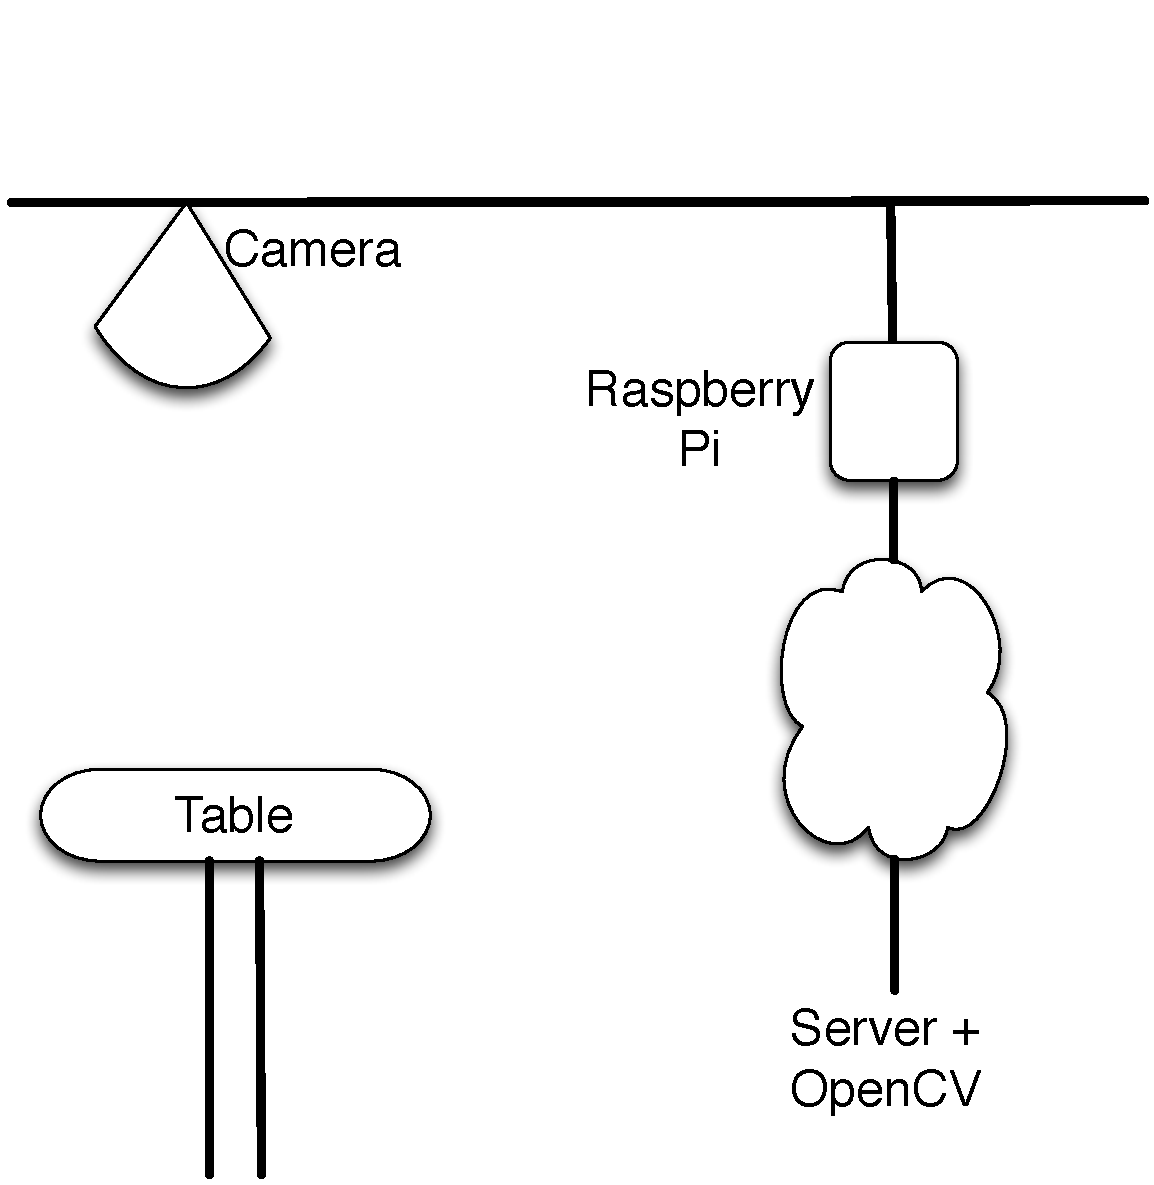
\includegraphics[width=0.3\textwidth]{./setup.pdf}
    \label{setup}
}
\hfill
\subfigure[]{
    \centering
    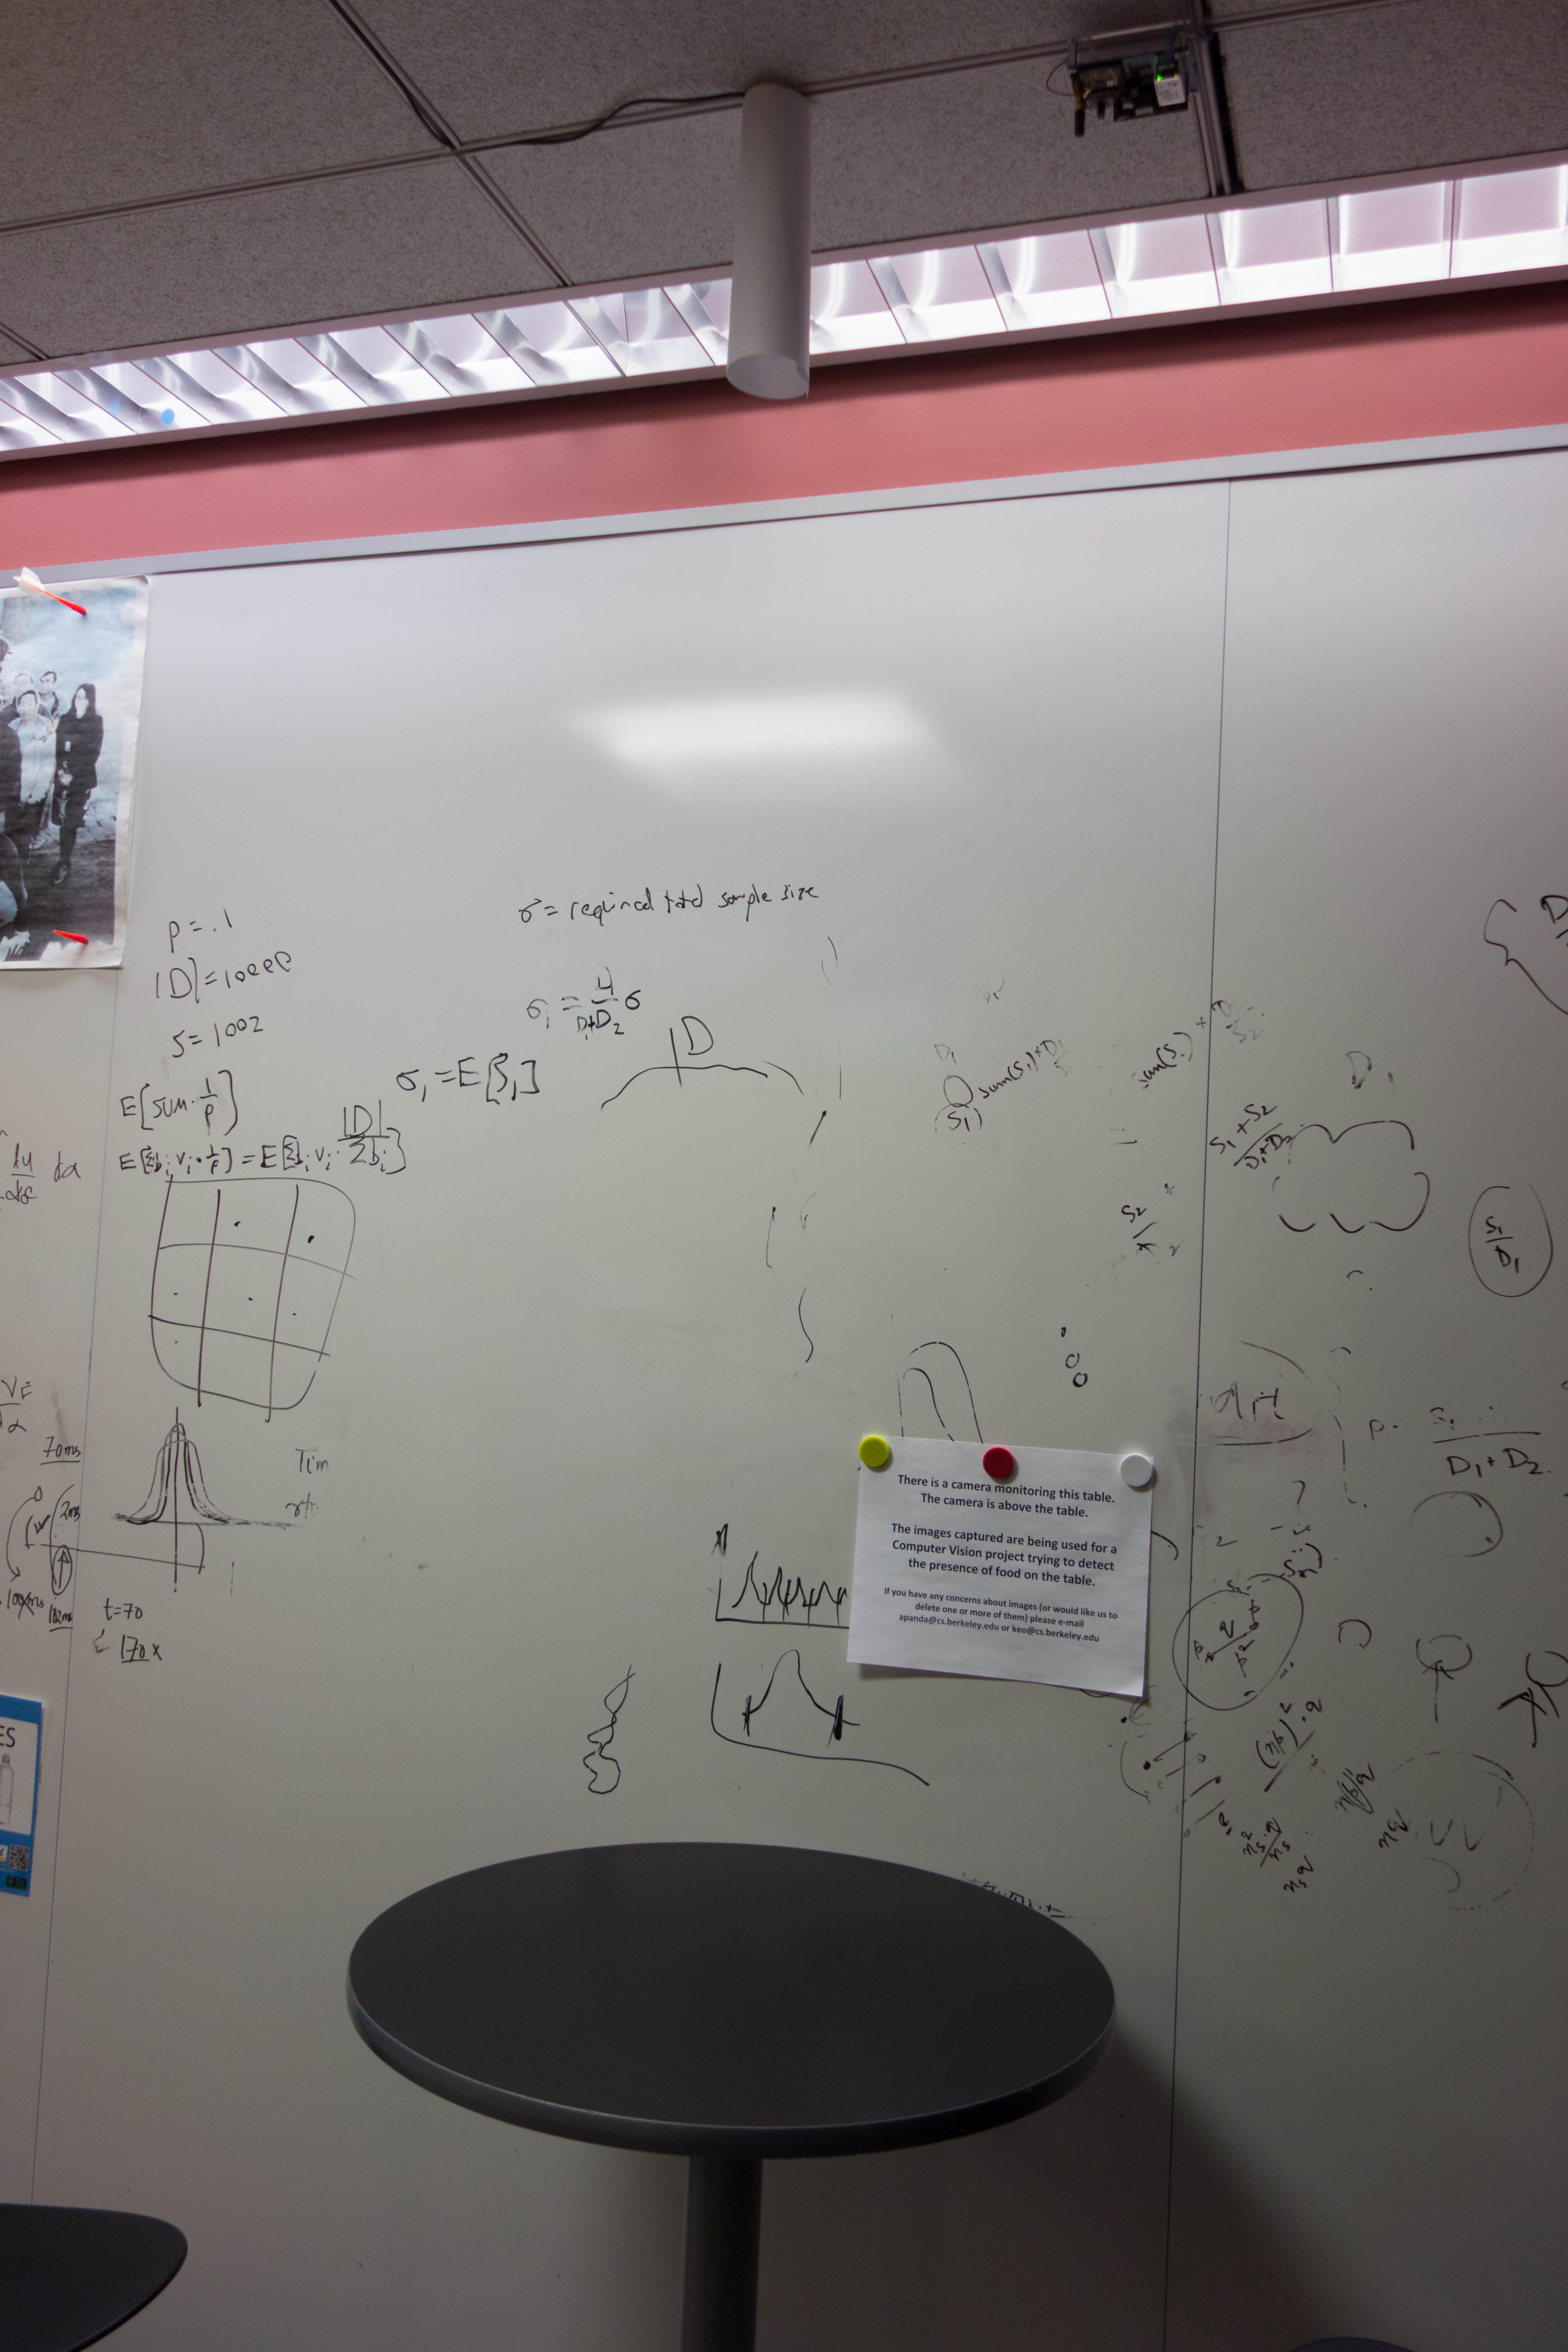
\includegraphics[width=0.3\textwidth]{./setup-real.jpg}
    \label{setup-real}
}
\caption[]{Acquisition setup \subref{setup} shows a schematic of our setup, \subref{setup-real} shows the actual setup in
the kitchen.}
\label{fig:acquisition}
\end{center}
\end{figure*}
The RADLab kitchen contains a single table on which all publicly edible food is placed. The kitchen also contains
various network ports (used to feed the printers) but does not have any computers. Our aim was to acquire images from
the table with minimal disruption. 

Our solution, which is shown in Figure~\ref{fig:acquisition}, relies on a compute to capture the images and a separate
computer for processing. We setup a camera and a Raspberry Pi~\cite{rpi} in the kitchen. Both of these can be discretely
placed in the kitchen. The Raspberry Pi is set to capture an image every $10$ seconds from the camera and runs a small
HTTP server that can serve this image. To minimize disk space and processing done on the Raspberry Pi, the image is
never written to disk and is served as a TIFF file. Every $30$ seconds a second computer in the AMPLab in the datacenter
polls the Raspberry Pi to acquire the latest image. The second computer is also responsible for running the detection
code on every image.


\begin{figure*}[!h]
\begin{center}
\subfigure[]{
    \centering
    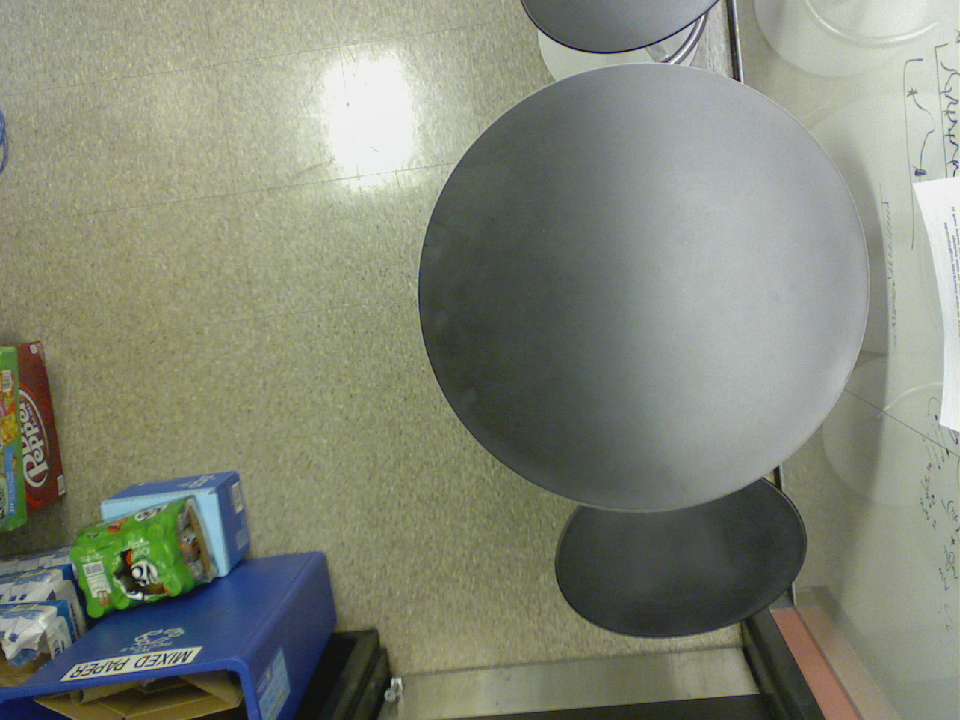
\includegraphics[width=0.3\textwidth]{./coneless.png}
    \label{coneless}
}
\hfill
\subfigure[]{
    \centering
    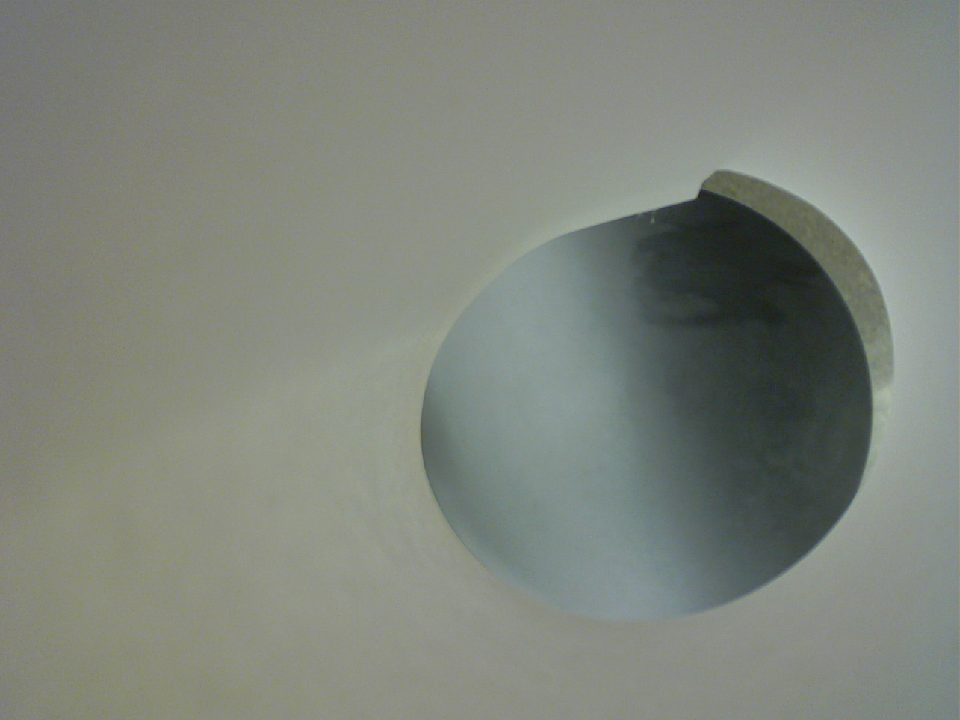
\includegraphics[width=0.3\textwidth]{./coned.png}
    \label{coned}
}
\caption[Input images]{\subref{coneless} full field of view, \subref{coned} limited view.}
\label{fig:input}
\end{center}
\end{figure*}
For privacy reasons we were required to place the camera in a manner that minimized the probability that it would
capture any humans. As a result we placed the camera vertically above the table resulting in images similar to
Figure~\ref{coneless}. To further limit the field of view (and hence simplify our problem somewhat) we added a paper
cone resulting in Figure~\ref{coned}. 

To train our SVM we collected $4$ days worth of images and hand labeled them. We then trained three different SVMs using
these images and the following feature vectors:
\begin{figure*}[!h]
\begin{center}
\subfigure[]{
    \centering
    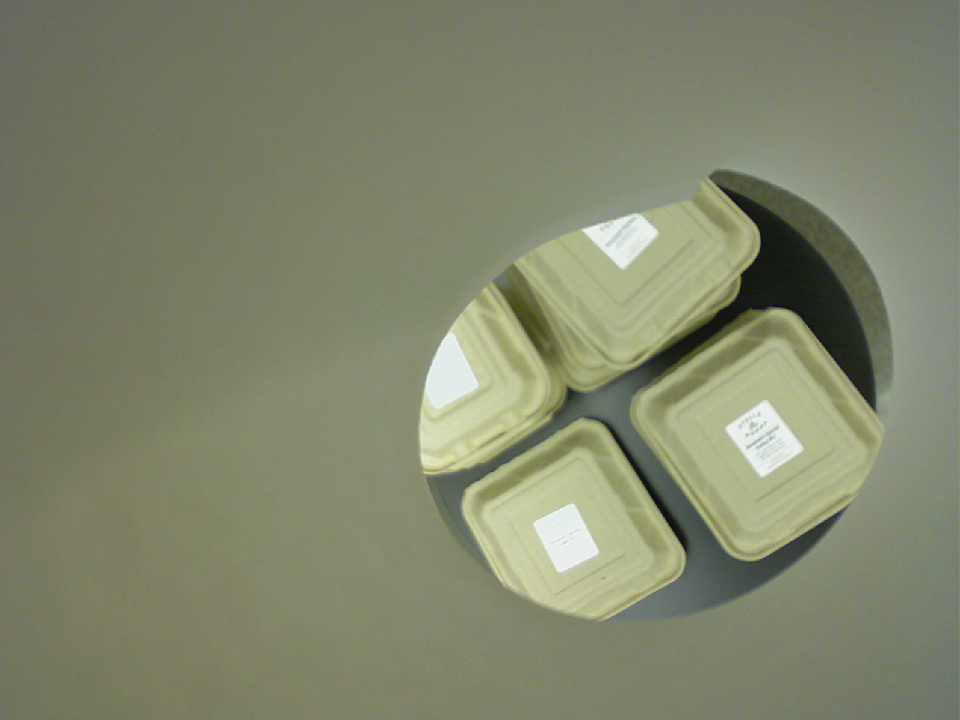
\includegraphics[width=0.3\textwidth]{./original-food.png}
    \label{fig:food-original}
}
\subfigure[]{
    \centering
    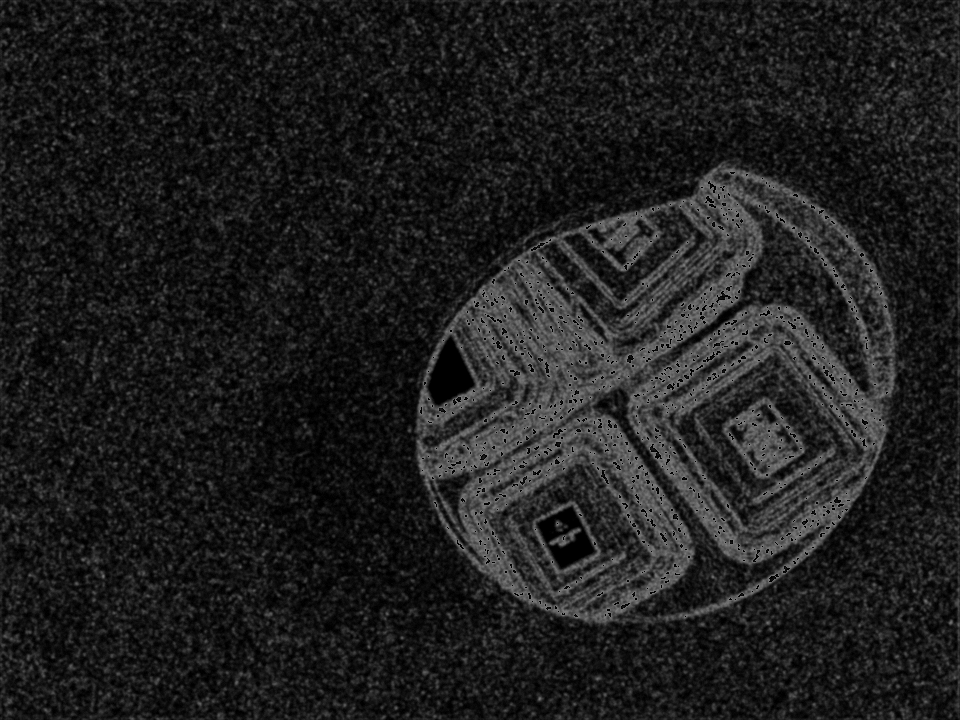
\includegraphics[width=0.3\textwidth]{./edge_food.png}
    \label{fig:food-edge}
}
\subfigure[]{
    \centering
    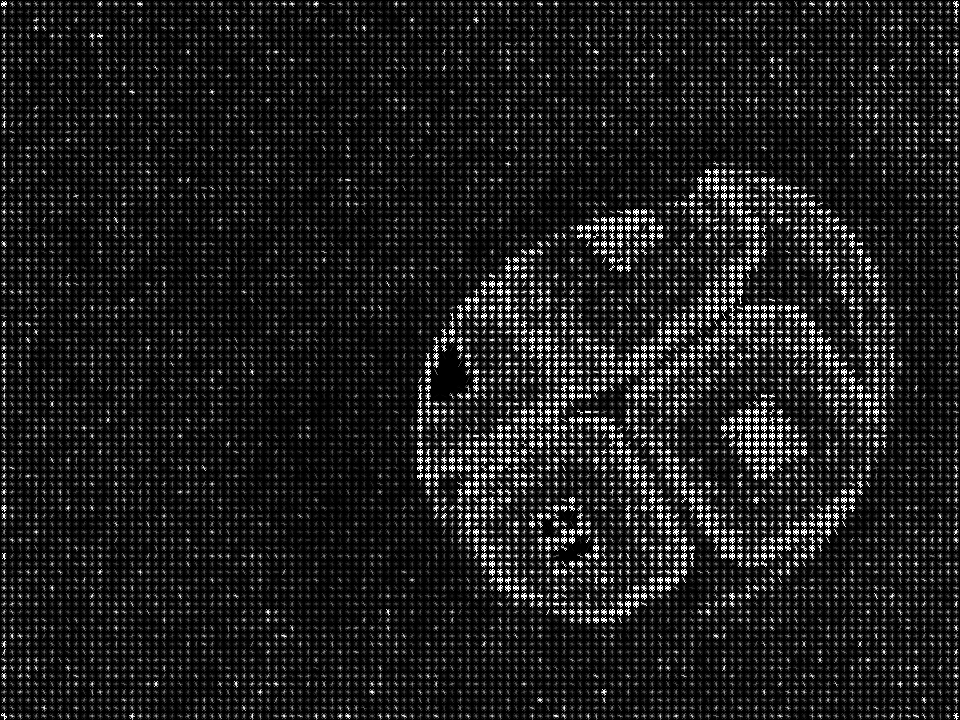
\includegraphics[width=0.3\textwidth]{./hog_vis_food.png}
    \label{fig:food-hog}
}
\caption[]{\subref{fig:food-original} Original image with food, \subref{fig:food-edge} with Shi Tomassi,
\subref{fig:food-hog} with HOG.}
\label{fig:food}
\end{center}
\end{figure*}
\begin{figure*}[!h]
\begin{center}
\subfigure[]{
    \centering
    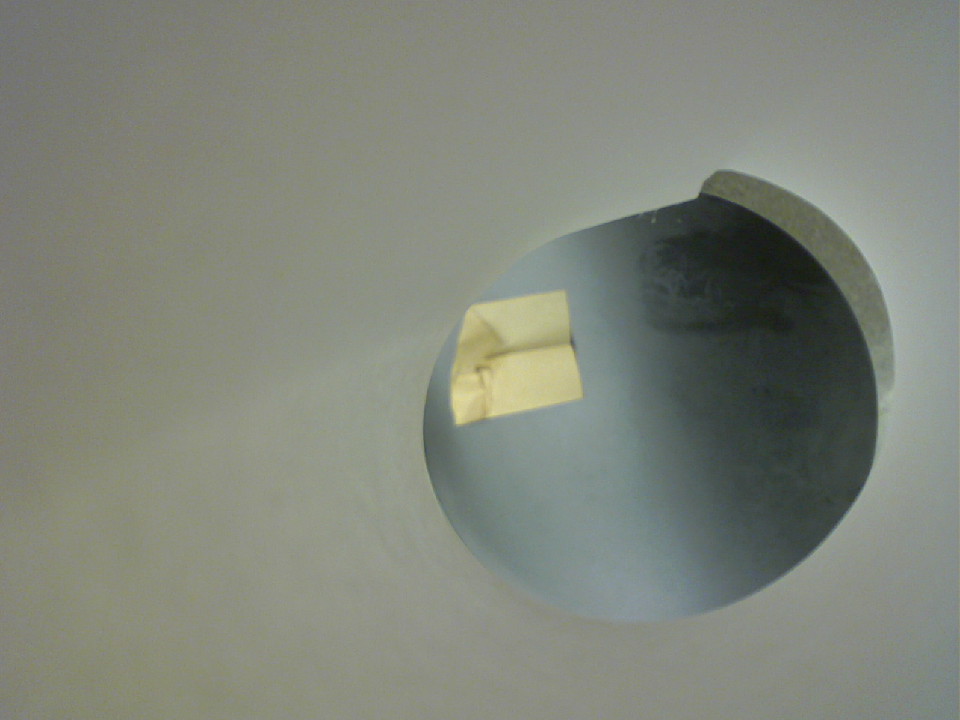
\includegraphics[width=0.3\textwidth]{./original-other.png}
    \label{fig:other-original}
}
\subfigure[]{
    \centering
    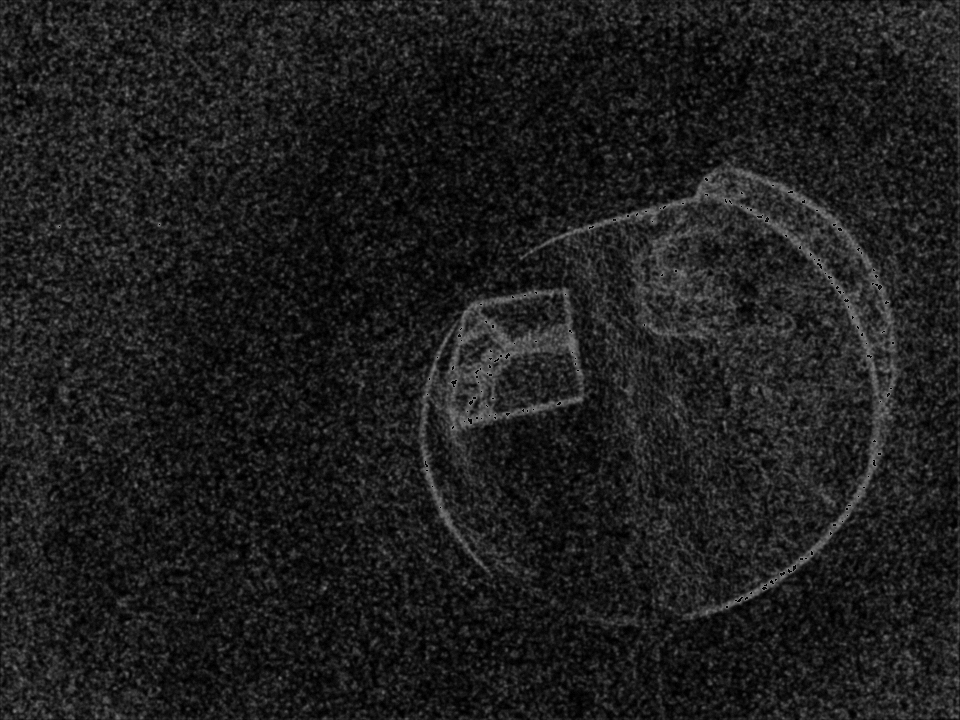
\includegraphics[width=0.3\textwidth]{./edge_vis_other.png}
    \label{fig:other-edge}
}
\subfigure[]{
    \centering
    
\includegraphics[width=0.3\textwidth]{./hog_vis_other.png}
    \label{fig:other-hog}
}
\caption[]{\subref{fig:other-original} Original image with other stuff, \subref{fig:other-edge} with Shi Tomassi,
\subref{fig:other-hog} with HOG.}
\label{fig:other}
\end{center}
\end{figure*}

\begin{figure*}[!h]
\begin{center}
\subfigure[]{
    \centering
    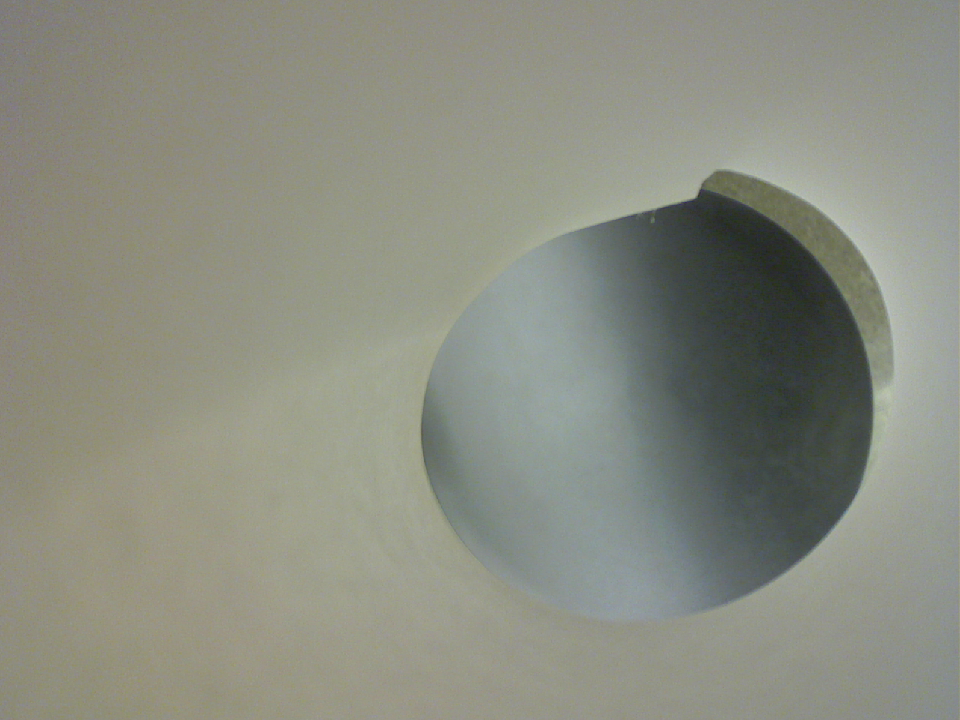
\includegraphics[width=0.3\textwidth]{./original-empty.png}
    \label{fig:empty-original}
}
\subfigure[]{
    \centering
    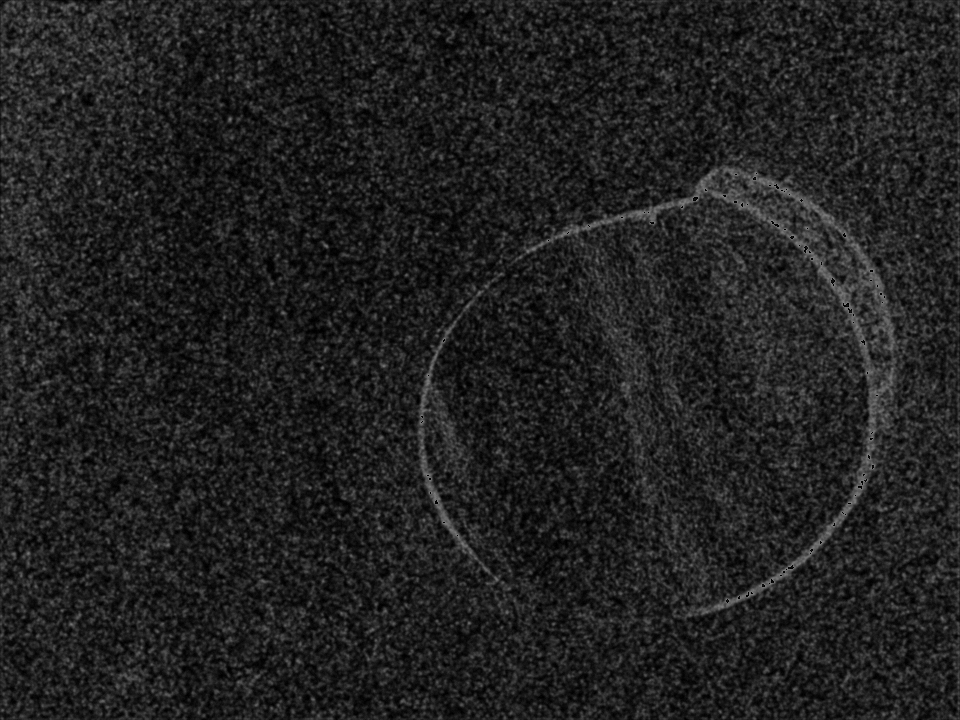
\includegraphics[width=0.3\textwidth]{./edge_vis_empty.png}
    \label{fig:empty-edge}
}
\subfigure[]{
    \centering
    
\includegraphics[width=0.3\textwidth]{./hog_vis_empty.png}
    \label{fig:empty-hog}
}
\caption[]{\subref{fig:empty-original} Original image of empty table, \subref{fig:empty-edge} with Shi Tomassi,
\subref{fig:empty-hog} with HOG.}
\label{fig:empty}
\end{center}
\end{figure*}
\begin{itemize}
\item The raw image after conversion to greyscale.
\item The image after edge/corner detection using Shi Tomassi~\cite{shi1994good}
\item Using HOG features.
\end{itemize}

Figures~\ref{fig:food},~\ref{fig:other},~\ref{fig:empty} show the feature vectors for a variety of cases.
